When analyzing the impact of FDI on wages and employment at the firm level, the  motive of the foreign investor might also play a role. For example, investors trying to sell their products in the destination country of their investment  may be particularly concerned about their reputation in the host country, potentially leading to higher wage payments. Our dataset also provides information on the type of FDI and distinguishes across four categories: exports-oriented FDI (1),  technology-intensive FDI (2), and domestic market seeking FDI (3). Of the firms receiving FDI, 44\% receive domestic-market seeking FDI, followed by 35\% that receive technology-intensive FDI. The share of firms receiving export-oriented FDI is 21\%. \\ \par

Figure \ref{fig_treatment_type} provides a graphical illustration of the main variables by type of FDI, displaying the means of wages, employment, TFP, export intensity and R\&D for 2015 and 2017, respectively. In addition, the graph displays the means for firms not receiving FDI (0). The corresponding Tables can be found in the Appendix (Tables \ref{sumstat_treatment_type_pre} and \ref{sumstat_treatment_type_post}). While the differences in means across types of FDI are relativley small when it comes to wages, employment, export intensity and TFP both in 2015 and 2017, the differences across FDI types are large regarding R\&D activities.\\ \par

 
\begin{figure}[htbp!]\caption{Pre- and post-treatment characteristics by treatment group}\label{fig_treatment_type}
	\begin{center}
		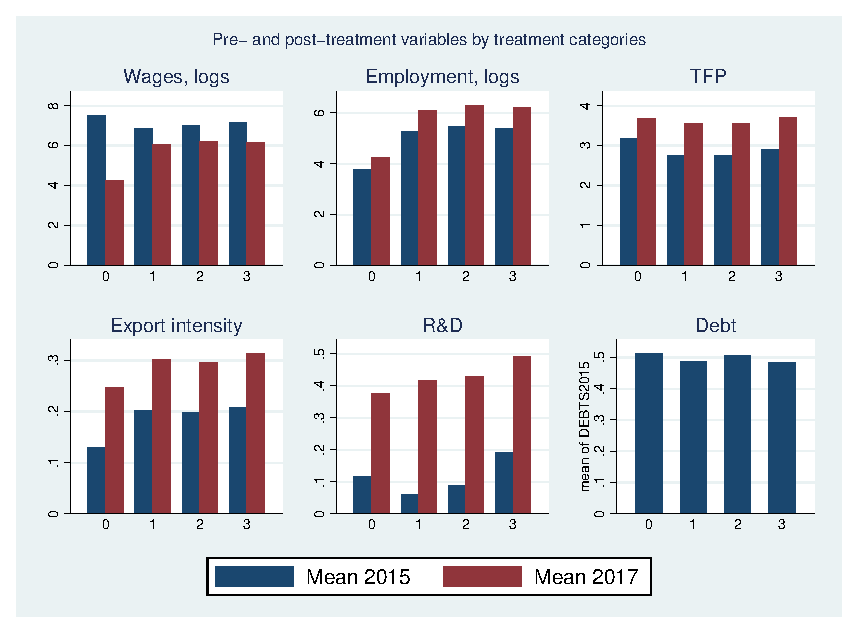
\includegraphics[scale=1]{figures_and_tables/bar_pre_post} 
	\end{center}
\end{figure}


With this knowledge in mind, we re-estimate the causal effects of FDI by type to examine if there are any differences in effects between types of FDI. Using the interacted scoring function specification, employed in Section 3, we find that the overlap improvements achieved in the previous section are found again evenly distributed of treatment types (compare Figure \ref{ol_aipw_type}). Thus, also with regard to FDI types it still remains partial as we do not manage to get a good overlap for propensity score values between 0 and 0.1. We test again IPW estimation performance given our suspicion that our treatment model is potentially incorrectly specified. As is the case in Section 3, the IPW estimator produces exceptionally large standard errors – an indication of possible misspecification in our treatment model. This is not the case for a linear model specification (excluding interaction effects), yet because balance improves when we use interactions in our model, we only estimate the interacted model for our further analysis (compare Tables \ref{bal_type_aipw} \& \ref{bal_type_ipw}). Given these findings, we rely on the AIPW estimates in this section as well.  

\begin{figure}
	\centering
	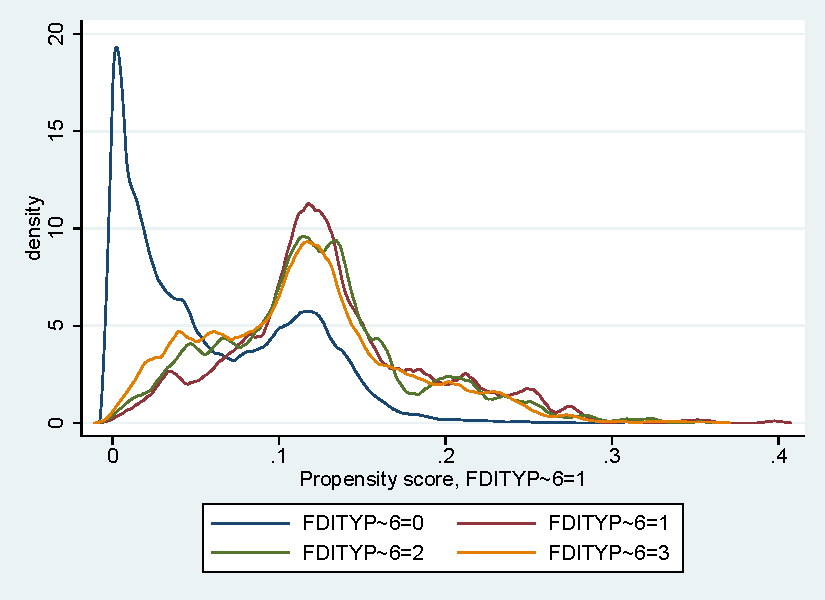
\includegraphics[scale=0.6]{figures_and_tables/4_overlap_aipw_typeFDI.pdf}\
	\caption{Overlap by type of treatment.}
	\label{ol_aipw_type}
\end{figure}

\begin{table}
	\def\sym#1{\ifmmode^{#1}\else\(^{#1}\)\fi}
	\caption{Causal effects of FDI (by type) on log employment}
	\label{4_table1}
	\begin{tabular}{l*{1}{cccc}}
		\hline\hline
		&\multicolumn{4}{c}{}                                        \\
		& (1) & (2) & (3)    \\
		\
		&ipw (no Interatcions) & ipw (interactions) & aipw (interactions)    \\
		\\
		&b/se&b/se& b/se       \\
		\hline
		\\
		ATE \\
		\\
		Export Oriented FDI &       0.73\sym{***} &  0.25  &   0.27\sym{***} \\
		&     (0.07)&     (0.42)&   (0.03)        \\
		Technology Intenstive FDI&       0.87\sym{***}&       0.59 &       0.28\sym{***}\\
		&     (0.08)&     (0.42)& (0.03)          \\
		Domestic Market Seeking FDI&       0.72\sym{***}&       0.21 &      0.27\sym{***}\\
		&     (0.06)&     (0.44)&     (0.03)   \\
		No FDI &       4.27\sym{***}&       4.27\sym{***} &      \sym{***}\\
		&     (0.03)&     (0.03)&     (0.03)   \\
		\hline
		\\
		Observations        &       11,323 &      11,318      &   11,318                  &            \\
		\hline\hline
		\\
		\small * p<0.1, ** p<0.05, *** p<0.01
	\end{tabular} \\
\end{table}



\begin{table}
	\def\sym#1{\ifmmode^{#1}\else\(^{#1}\)\fi}
	\centering
	\caption{Causal effects of FDI (by type) on log wages}
	\label{4_table2}
	\begin{tabular}{l*{1}{cccc}}
		\hline\hline
		&\multicolumn{1}{c}{}                                        \\
		& (1)   \\
		\
		&aipw (interactions)     \\
		\\
		&b/se       \\
		\hline
		\\
		ATE \\
		\\
		Export Oriented FDI &       0.21\sym{***}   \\
		&     (0.02)        \\
		Technology Intenstive FDI&       0.22\sym{***} \\
		&     (0.03)         \\
		Domestic Market Seeking FDI&       0.23\sym{***}\\
		&     (0.02)   \\
		No FDI&       4.93\sym{***}\\
		&     (0.03)   \\
		\hline
		\\
		Observations        & 11,318          
		&                 &            \\
		\hline\hline
		\\
		\small * p<0.1, ** p<0.05, *** p<0.01
	\end{tabular} \\
\end{table}


Table \ref{4_table1} shows that for all the types of FDI the average treatment effect is the same. The coefficient estimated by the AIPW estimator for employment is 0.27 - 0.28 when compared to firms which do not have any FDI at all. The average log employment of the untreated is estimated to be 4.9. For wages, we observe the same trend, shown in Table \ref{4_table2}. The ATE for export-oriented, technology-intensive FDIs and domestic market seeking FDIs being 0.21-0.23, with the average log wages value for the non-treated firm is 4.9. 

